% Created 2024-06-01 Sat 11:22
% Intended LaTeX compiler: pdflatex
\documentclass[presentation,aspectratio=169,smaller]{beamer}
\usepackage[utf8]{inputenc}
\usepackage[T1]{fontenc}
\usepackage{graphicx}
\usepackage{longtable}
\usepackage{wrapfig}
\usepackage{rotating}
\usepackage[normalem]{ulem}
\usepackage{amsmath}
\usepackage{amssymb}
\usepackage{capt-of}
\usepackage{hyperref}
\usepackage{color}
\usepackage[newfloat]{minted}
\usepackage[utf8]{inputenc}
\usepackage{soul}
\usepackage{unicode-math}
\usepackage{mathtools}
\usepackage[mathletters]{ucs}
\usemintedstyle{tango}
\setminted{fontsize=\scriptsize}
\setminted{mathescape=true}
\setbeamertemplate{itemize items}[circle]
\setbeamertemplate{enumerate items}[default]
\setlength{\parskip}{\baselineskip}%
\setlength{\parindent}{0pt}%
\setbeamertemplate{navigation symbols}{}%remove navigation symbols
\newcommand{\hlyellow}[1]{\colorbox{yellow!50}{$\displaystyle#1$}}
\newcommand{\hlfancy}[2]{\sethlcolor{#1}\hl{#2}}
\usetheme{default}
\author{Boris Buliga}
\date{June 01, 2024}
\title{Drinking wine with Emacs}
\subtitle{or a story of technical alcoholism}
\hypersetup{
 pdfauthor={Boris Buliga},
 pdftitle={Drinking wine with Emacs},
 pdfkeywords={},
 pdfsubject={},
 pdfcreator={Emacs 30.0.50 (Org mode 9.7-pre)}, 
 pdflang={English}}
\begin{document}

\maketitle
\newcommand{\mathcolorbox}[2]{%
  \begingroup
  \setlength{\fboxsep}{2pt}%
  \colorbox{#1}{$\displaystyle #2$}%
  \endgroup
}

\AtBeginSection[]{
  \begin{frame}
  \vfill
  \centering
  \begin{beamercolorbox}[sep=8pt,center,shadow=true,rounded=true]{title}
    \usebeamerfont{title}\insertsectionhead\par%
  \end{beamercolorbox}
  \vfill
  \end{frame}
}
\section*{Intro}
\label{sec:orgd50c1a8}
\begin{frame}[label={sec:orgd6c33a0}]{Frequently Asked Questions}
\begin{itemize}
\item Can I get a replacement for my broken glass?
\item What is the difference between Pét-Nat and Method Ancestrale?
\item Where is Nadia Verrua?
\item What the heck is Emacs?
\item Why does Mykola hate dosage in Champagne?
\end{itemize}
\end{frame}
\begin{frame}[label={sec:org10c9c75}]{Broken glass?}
\begin{center}
\includegraphics[height=5.5cm]{images/defeated-male.jpg}
\end{center}
\end{frame}
\begin{frame}[label={sec:orgdf6f171},fragile]{What the heck is Emacs?\footnote{I still ask myself this very question.}}
 \begin{columns}
\begin{column}{0.5\columnwidth}
\begin{itemize}
\item \alert{Extensible} text editor.
\item Development began in 1970s.
\item Initially released in 1976.
\item Actively maintained till this day.
\item Use \texttt{C-x C-c} to quit it.
\item It's like Notepad/TextEdit, but for nerdy and masochistic kids.
\item It's counter-intuitive, but some people do in fact love Emacs.
\end{itemize}
\end{column}
\begin{column}{0.5\columnwidth}
\begin{center}
\includegraphics[height=3.5cm]{images/emacs.png}
\end{center}
\end{column}
\end{columns}
\end{frame}
\begin{frame}[label={sec:org9a9e568}]{Order salads}
\begin{figure}[htbp]
\centering
\includegraphics[height=5.0cm]{images/salad.png}
\caption{from \texttt{CestDiego/sweetgreen.el}}
\end{figure}
\end{frame}
\begin{frame}[label={sec:org95f9905}]{Read email}
\begin{figure}[htbp]
\centering
\includegraphics[height=7.0cm]{images/email-dashboard.png}
\caption{from \texttt{rougier/mu4e-dashboard}}
\end{figure}
\end{frame}
\begin{frame}[label={sec:org5a566c7}]{Control sex toys}
\begin{figure}[htbp]
\centering
\includegraphics[height=5.0cm]{images/deldo.png}
\caption{You may like Emacs, but Kyle (aka Poor Life Choices) \textbf{loves} Emacs. And it's mutual.}
\end{figure}
\end{frame}
\begin{frame}[label={sec:orge60ea4b}]{Write some code}
\begin{center}
\includegraphics[height=8.0cm]{images/coding.png}
\end{center}
\end{frame}
\begin{frame}[label={sec:org17b0f21}]{Take notes and manage tasks}
\begin{center}
\includegraphics[height=8.0cm]{images/note-taking.png}
\end{center}
\end{frame}
\begin{frame}[label={sec:orgc868b6f}]{Manage your wine cellar}
\begin{center}
\includegraphics[height=8.0cm]{images/wine-notes.png}
\end{center}
\end{frame}
\begin{frame}[label={sec:orge457b70}]{About me}
\begin{columns}
\begin{column}{0.75\columnwidth}
\begin{itemize}
\item Server Guild Manager @Wix.
\item Author of Barberry Garden.
\item Wine enthusiast.
\begin{itemize}
\item Not a sommelier.
\item No affiliations with wine importers or stores.
\end{itemize}
\item Emacs user for 10+ years.
\end{itemize}
\end{column}
\begin{column}{0.25\columnwidth}
\begin{figure}[htbp]
\centering
\includegraphics[height=3.5cm]{images/boris.jpg}
\caption{Boris Buliga}
\end{figure}
\end{column}
\end{columns}
\end{frame}
\section{I drink wine}
\label{sec:org6f3293b}

\begin{frame}[label={sec:orge124827}]{I \sout{love} need\footnote{Is it Obsessive-compulsive disorder? Nah, it's just my crappy memory.} to take notes}
\begin{enumerate}
\item Information about wine, producer, region, grape, technology, etc.
\item Score and tasting notes.
\item What, when, where and with whom.
\item Manage cellar.
\end{enumerate}
\end{frame}
\section{Existing solutions}
\label{sec:orgb19199f}
\begin{frame}[label={sec:org5bb3e63}]{Vivino: Buy The Right Wine}
\begin{columns}
\begin{column}{0.6\columnwidth}
\begin{itemize}
\item An online wine marketplace and wine app.
\item Launched in 2010.
\item Arguably the most popular wine application on [UA] market.
\item AFAIK devs are located in Lviv.
\item Premium is not required.
\end{itemize}
\end{column}
\begin{column}{0.4\columnwidth}
\begin{center}
\includegraphics[height=7.0cm]{images/vivino.png}
\end{center}
\end{column}
\end{columns}
\end{frame}
\begin{frame}[label={sec:org09f83c3}]{Vivino Pros}
\begin{columns}
\begin{column}{0.5\columnwidth}
\begin{itemize}
\item Huge user base. Including folks from UA.
\item Huge wine base.
\item Can't find a wine? Add it yourself.
\item Good image recognition.
\item Simple cellar tracking.
\item Taste profile.
\item Wine Adventures.
\end{itemize}
\end{column}
\begin{column}{0.25\columnwidth}
\begin{center}
\includegraphics[height=7.0cm]{images/vivino-adventures.png}
\end{center}
\end{column}
\begin{column}{0.25\columnwidth}
\begin{center}
\includegraphics[height=7.0cm]{images/vivino-taste-profile.png}
\end{center}
\end{column}
\end{columns}
\end{frame}
\begin{frame}[label={sec:orga7ae0c7}]{Vivino Cons}
\begin{columns}
\begin{column}{1.0\columnwidth}
\begin{itemize}
\item Mostly useless ratings.
\begin{itemize}
\item Subscribe to people you trust.
\end{itemize}
\item Duplicated wines and mistakes.
\item Strict limit on review length (\(2^9\) characters).
\item Buggy and sometimes too eventual "eventual consistency".
\item Mostly useless premium. But at least you support folks.
\item Lame Web version.
\item No export functionality.
\item User ranking and achievements.
\end{itemize}
\end{column}
\end{columns}
\end{frame}
\begin{frame}[label={sec:orgd6657c5}]{User Ranking and Achievements}
\begin{columns}
\begin{column}{0.3\columnwidth}
\begin{center}
\includegraphics[height=7.0cm]{images/vivino-rank.png}
\end{center}
\end{column}
\begin{column}{0.3\columnwidth}
\begin{center}
\includegraphics[height=7.0cm]{images/vivino-achievements.png}
\end{center}
\end{column}
\begin{column}{0.3\columnwidth}
\begin{itemize}
\item Gamification
\item Forces interactions
\item Promotes users
\end{itemize}
\end{column}
\end{columns}
\end{frame}
\begin{frame}[label={sec:org8da8133}]{User Ranking and Achievements}
\begin{columns}
\begin{column}{0.4\columnwidth}
It promotes

\begin{itemize}
\item unhealthy \alert{habits}
\item unhealthy \alert{culture}
\end{itemize}
\end{column}
\begin{column}{0.6\columnwidth}
\begin{center}
\includegraphics[height=6.0cm]{images/fry-coffee.jpg}
\end{center}
\end{column}
\end{columns}
\end{frame}
\begin{frame}[label={sec:orgc187ed2}]{Delectable - Scan \& Rate Wine}
\begin{columns}
\begin{column}{0.6\columnwidth}
\begin{itemize}
\item A platform to share and discover wine.
\item Launched in 2011.
\item Run by Vinous Group.
\begin{itemize}
\item Don't forget to subscribe.
\end{itemize}
\item Premium is not required.
\end{itemize}
\end{column}
\begin{column}{0.4\columnwidth}
\begin{center}
\includegraphics[height=7.0cm]{images/delectable.png}
\end{center}
\end{column}
\end{columns}
\end{frame}
\begin{frame}[label={sec:org9dd831a}]{Delectable Pros}
\begin{columns}
\begin{column}{0.5\columnwidth}
\begin{itemize}
\item Active user base, but smaller compared to Vivino.
\item Decent wine base.
\item Less strict limits on the review length.
\item No user ranking.
\item Nice users promotion approach.
\item Ok Web version.
\end{itemize}
\end{column}
\begin{column}{0.25\columnwidth}
\begin{center}
\includegraphics[height=7.0cm]{images/delectable-home.png}
\end{center}
\end{column}
\begin{column}{0.25\columnwidth}
\begin{center}
\includegraphics[height=7.0cm]{images/delectable-trending.png}
\end{center}
\end{column}
\end{columns}
\end{frame}
\begin{frame}[label={sec:orge8f9f3c}]{Delectable Cons}
\begin{columns}
\begin{column}{0.5\columnwidth}
\begin{itemize}
\item Can't find wine?
\begin{itemize}
\item Someone from the team will process it and create a new wine entry if needed.
\item Premium gives priority wine transcription.
\item The team can't figure it out? Too bad.
\end{itemize}
\item Almost no users from UA.
\item No cellar feature.
\item Lame taste insights.
\item No export functionality.
\end{itemize}
\end{column}
\begin{column}{0.25\columnwidth}
\begin{center}
\includegraphics[height=7.0cm]{images/delectable-missing-wines.png}
\end{center}
\end{column}
\begin{column}{0.25\columnwidth}
\begin{center}
\includegraphics[height=7.0cm]{images/delectable-taste-insights.png}
\end{center}
\end{column}
\end{columns}
\end{frame}
\begin{frame}[label={sec:org8cbbd75}]{CellarTracker - Wine Reviews \& Cellar Management Tools}
\begin{itemize}
\item A platform for cellar management and note taking.
\item Launched in 2003.
\item Premium is optional.
\item A bit old school.
\end{itemize}
\end{frame}
\begin{frame}[label={sec:orgc743fd7}]{Dial-up vibes}
\begin{center}
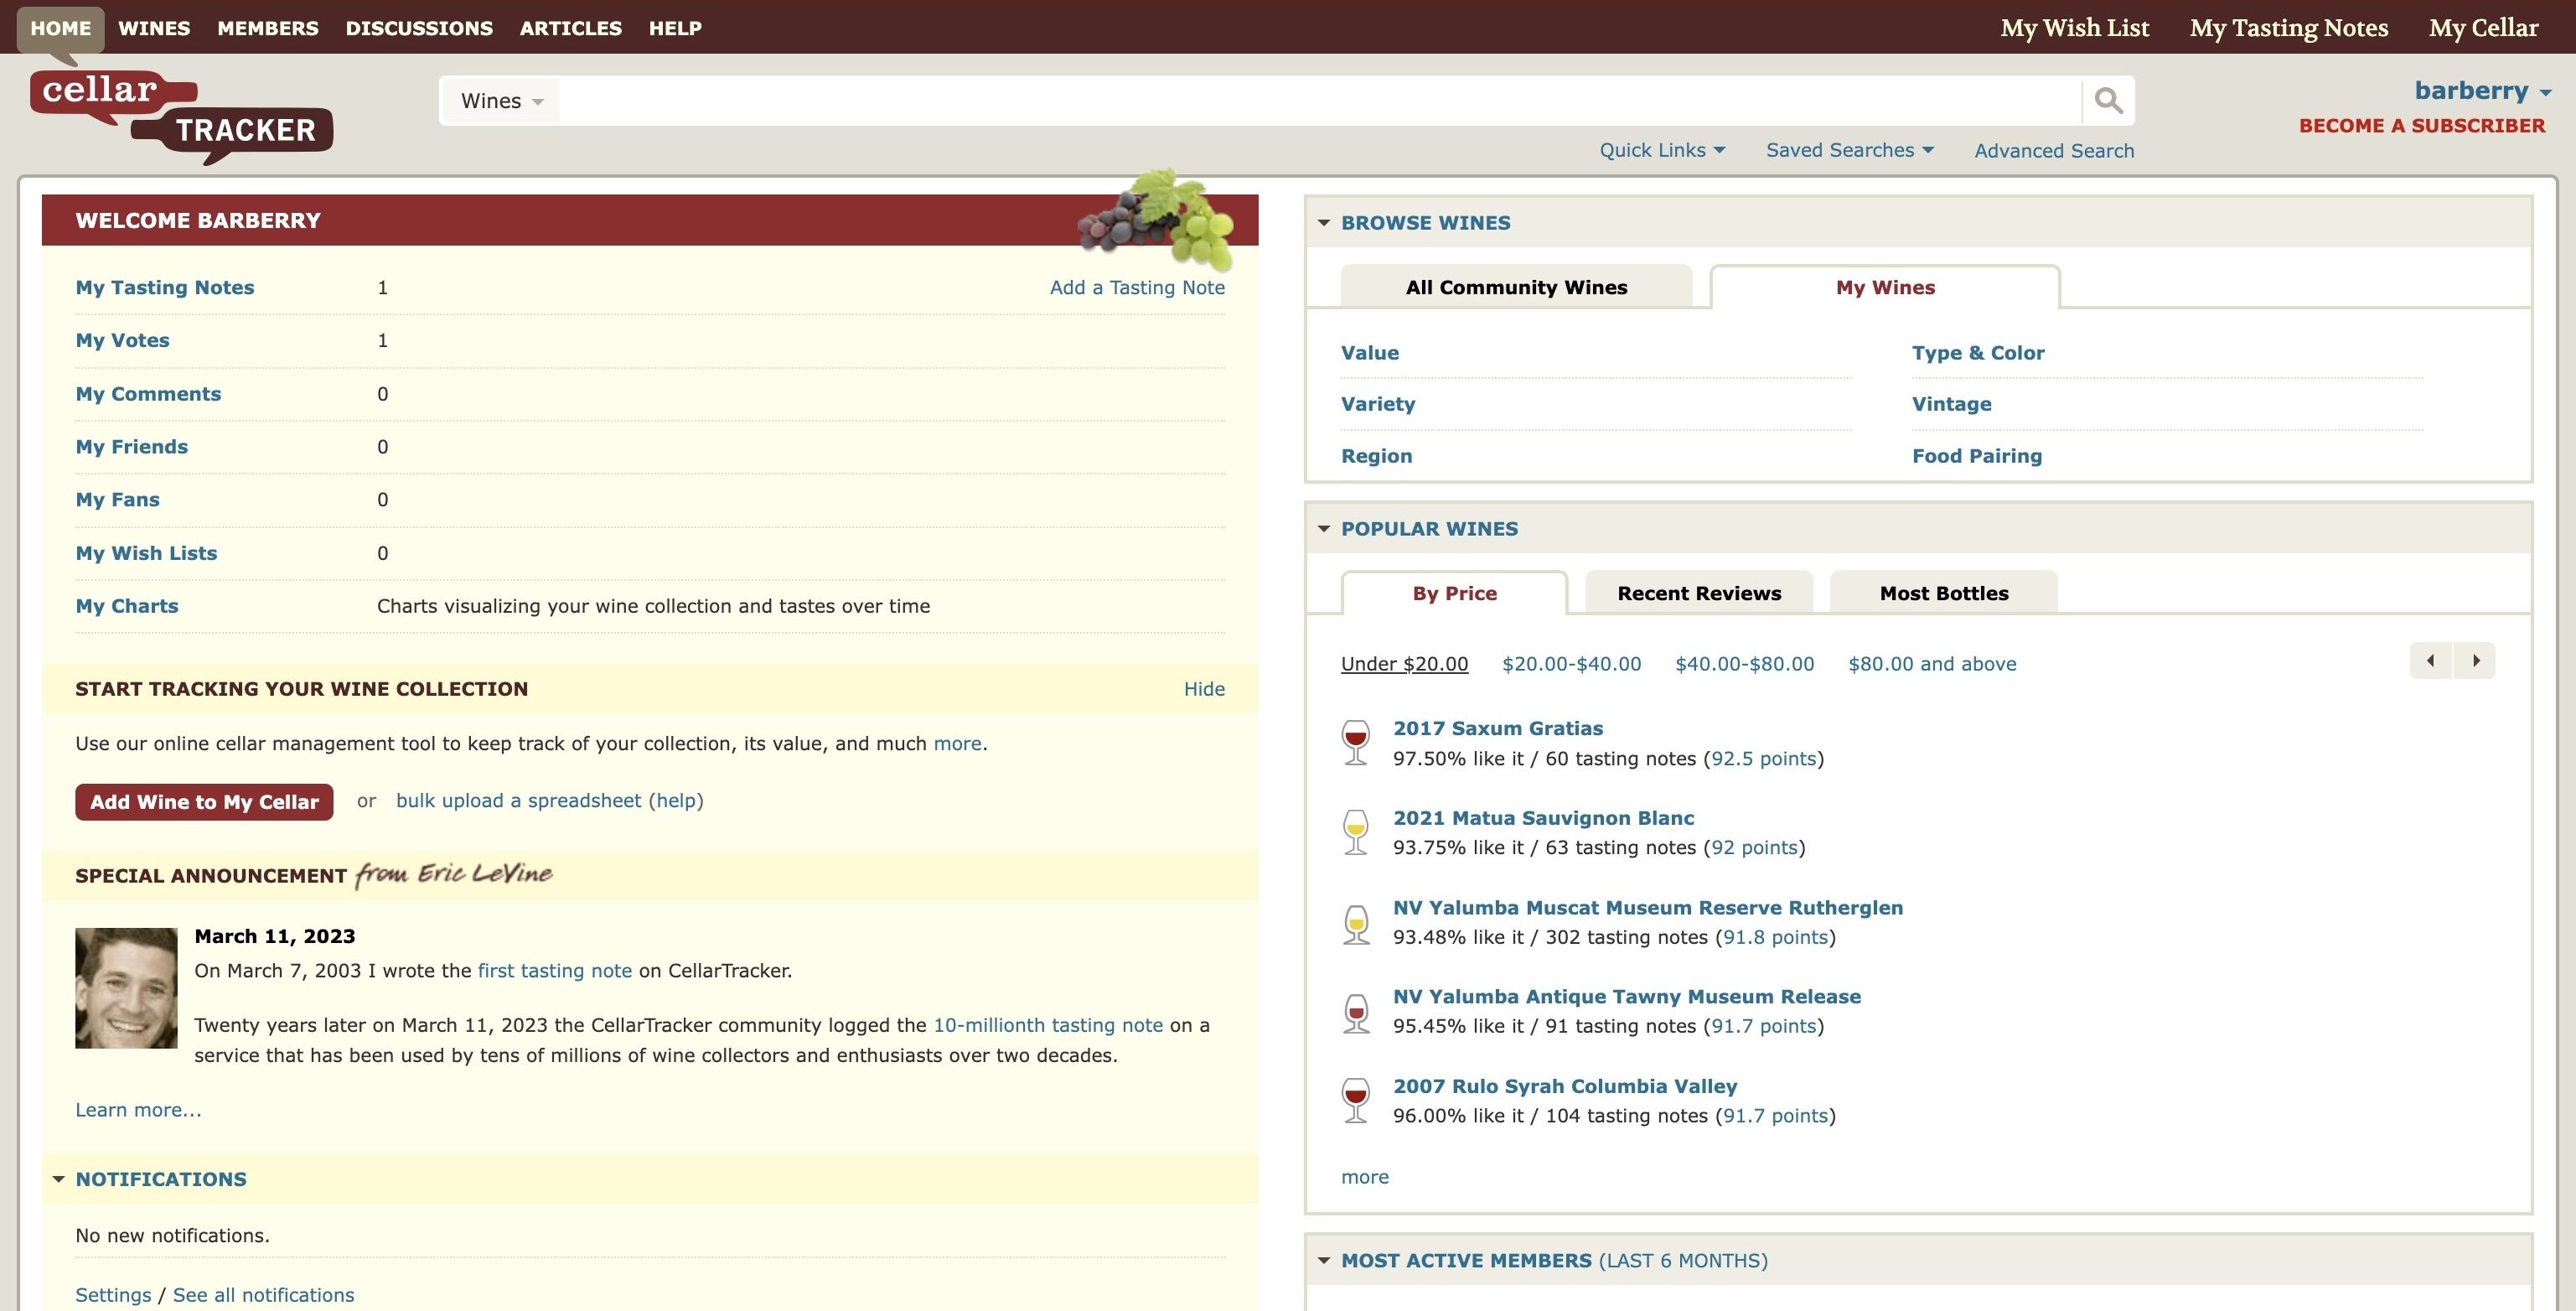
\includegraphics[height=7.0cm]{images/cellar-tracker-home-desktop.jpeg}
\end{center}
\end{frame}
\begin{frame}[label={sec:org4e85506}]{Dial-up vibes\ldots{}}
\begin{center}
\includegraphics[height=6.0cm]{images/cellar-tracker-mobile-1.png}
\end{center}
\end{frame}
\begin{frame}[label={sec:org65884ca}]{A fresh face}
\begin{columns}
\begin{column}{0.5\columnwidth}
\begin{figure}[htbp]
\centering
\includegraphics[height=6.0cm]{images/cellar-tracker-mobile-1.png}
\caption{before}
\end{figure}
\end{column}
\begin{column}{0.5\columnwidth}
\begin{figure}[htbp]
\centering
\includegraphics[height=6.0cm]{images/cellar-tracker-mobile-2.png}
\caption{after}
\end{figure}
\end{column}
\end{columns}
\end{frame}
\begin{frame}[label={sec:orgfc551d2}]{A fresh new face}
\begin{center}
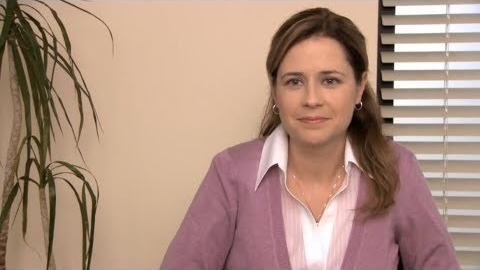
\includegraphics[height=7.0cm]{images/theare-the-same.jpeg}
\end{center}
\end{frame}
\begin{frame}[label={sec:orgb0d91c3}]{CellarTracker Pros}
\begin{columns}
\begin{column}{0.5\columnwidth}
\begin{itemize}
\item A small but active user base.
\item Huge wine base.
\item Easy to add new wine records and edit mistakes.
\item The most advanced cellar tracker capabilities.
\item The most advanced note taking capabilities.
\item Full-blown web version.
\item Good image recognition (based on Vivino).
\item Data export functionality.
\end{itemize}
\end{column}
\begin{column}{0.25\columnwidth}
\begin{center}
\includegraphics[height=7.0cm]{images/cellar-tracker-add-bottle-1.png}
\end{center}
\end{column}
\begin{column}{0.25\columnwidth}
\begin{center}
\includegraphics[height=7.0cm]{images/cellar-tracker-add-bottle-2.png}
\end{center}
\end{column}
\end{columns}
\end{frame}
\begin{frame}[label={sec:org0d1a727}]{CellarTracker Cons}
\begin{itemize}
\item \sout{UI}
\item Complexity.
\item 67 users from UA.
\begin{itemize}
\item 5 users with >100 reviews.
\end{itemize}
\end{itemize}
\end{frame}
\section{And the winner is\ldots{}}
\label{sec:orge6479ee}

\begin{frame}[label={sec:org43deb33}]{No one, really}
\begin{itemize}
\item Vivino is leader because of community.
\item I wish Delectable didn't fail in the core feature.
\item CellarTracker is superior, obviously.
\end{itemize}
\end{frame}
\begin{frame}[label={sec:org8911b9f}]{So what's wrong?}
\begin{enumerate}
\item Data is not owned by me.
\item Incorrect data.
\item No way to extend data with extra fields.
\item Capabilities limited by proprietary solution.
\item Requires internet connection (and who is laughing now?).
\item \ldots{}
\item I am engineer, I am capable of creating my own solution.
\end{enumerate}
\end{frame}
\begin{frame}[label={sec:org31039ba}]{What are my options?}
\begin{itemize}
\item Notebooks (plain and specialised)
\item Spreadsheets
\item AirTable
\item Notion
\item <2-> Emacs
\end{itemize}
\end{frame}
\begin{frame}[label={sec:org29c2817}]{Obviously\ldots{}}
\begin{center}
\includegraphics[height=3.5cm]{images/emacs.png}
\end{center}

\begin{quote}
Solution? \sout{Kafka} Emacs.

Problem? You tell me.

--- a wise man
\end{quote}
\end{frame}
\begin{frame}[label={sec:org5e7ecaf}]{Important aspects}
\begin{itemize}
\item Evolutionary approach
\item Automation
\item Fun
\end{itemize}
\end{frame}
\section{Emacs as a wine app}
\label{sec:org0c500af}

\begin{frame}[label={sec:org3f1ce96}]{Org Mode for the rescue}
\begin{columns}
\begin{column}{0.75\columnwidth}
\begin{itemize}
\item A markup language (like markdown, but beefed with features).
\item An extension for Emacs.
\item Provides nice APIs to manipulate documents.
\item People use it to write documents, notes, presentations manage tasks and projects, etc.
\end{itemize}
\end{column}
\begin{column}{0.25\columnwidth}
\begin{center}
\includegraphics[height=3.5cm]{images/org-mode-unicorn.png}
\end{center}
\end{column}
\end{columns}
\end{frame}
\begin{frame}[label={sec:orgbfa8082}]{What the actual heck?}
\begin{center}
\includegraphics[height=7.0cm]{images/org-mode-example.png}
\end{center}
\end{frame}
\begin{frame}[label={sec:org4b2d72d}]{It can be less ugly\ldots{} probably}
\begin{center}
\includegraphics[height=8.0cm]{images/org-mode-example-2.png}
\end{center}
\end{frame}
\begin{frame}[label={sec:org2da3899}]{Notes structure}
\begin{center}
\includegraphics[height=7.0cm]{images/notes-structure.png}
\end{center}
\end{frame}
\begin{frame}[label={sec:orgc6934ac}]{Wine entry}
\begin{center}
\includegraphics[height=8.0cm]{images/vino-wine-entry.png}
\end{center}
\end{frame}
\begin{frame}[label={sec:orgaa6f670}]{Rating}
\begin{center}
\includegraphics[height=8.0cm]{images/vino-rating.png}
\end{center}
\end{frame}
\begin{frame}[label={sec:org82f4384},fragile]{Database}
 \begin{itemize}
\item All notes (e.g. data) are structured.
\item There are APIs to parse these notes.
\item So it's easy to build a database (\texttt{sqlite}) from the notes.
\end{itemize}

\begin{center}
\includegraphics[height=5.0cm]{images/database.png}
\end{center}
\end{frame}
\begin{frame}[label={sec:orge77d27d}]{Vulpea}
\begin{columns}
\begin{column}{0.75\columnwidth}
\begin{itemize}
\item A collection of functions for note taking based on Org Mode and Org Roam.
\item A library to write applications and utilities around Org notes (structured or not).
\item Optimized for reads.
\item Allows to query by different metadata, custom fields, links etc.
\item Allows to extend database with custom tables and data extractors.
\item Handles quite big notes collection (50k+).
\item \url{https://github.com/d12frosted/vulpea}
\end{itemize}
\end{column}
\begin{column}{0.25\columnwidth}
\begin{center}
\includegraphics[height=3.5cm]{images/vulpea.png}
\end{center}
\end{column}
\end{columns}
\end{frame}
\begin{frame}[label={sec:org998a34d}]{Vino}
\begin{columns}
\begin{column}{0.75\columnwidth}
\begin{itemize}
\item An Emacs application for cellar tracking and wine notes management.
\item \url{https://github.com/d12frosted/vino}
\end{itemize}
\end{column}
\begin{column}{0.25\columnwidth}
\begin{center}
\includegraphics[height=3.5cm]{images/vino.png}
\end{center}
\end{column}
\end{columns}
\end{frame}
\begin{frame}[label={sec:orge1733a3}]{So what?}
\begin{itemize}
\item I have org files as source of truth. These notes are \alert{well-structured}.
\item I have APIs to manipulate these files.
\item I have database with all data extracted (so there is no need to parse these files every time).
\end{itemize}
\end{frame}
\section{Emacs UI is ugly, isn't it? And no one can read your notes.}
\label{sec:orgf117d86}

\begin{frame}[label={sec:org84f95ec}]{\url{https://barberry.io}}
\begin{center}
\includegraphics[height=8.0cm]{images/barberry-garden-home.png}
\end{center}
\end{frame}
\begin{frame}[label={sec:orgc3b134f}]{publicatorg}
\begin{center}
\includegraphics[height=8.0cm]{images/publicatorg.png}
\end{center}
\end{frame}
\begin{frame}[label={sec:orga9ffe78}]{publicatorg}
\begin{center}
\includegraphics[height=8.0cm]{images/publicatorg-exec.png}
\end{center}
\end{frame}
\begin{frame}[label={sec:org70ac26b}]{And it's crazy cool}
\begin{itemize}
\item I can keep my private notes as the source of truth.
\item I have my cozy Emacs UI.
\item But thanks to structured notes and APIs I can build multiple views.
\item \ldots{}
\item Just think about it :) I am overly excited!
\end{itemize}
\end{frame}
\section{Some cool features}
\label{sec:org770dc60}

\begin{frame}[label={sec:org8f72928}]{CellarTracker}
Me: can we have a CellarTracker?\\
Mom: we have CellarTracker at home.\\
CellarTracker at home:

\begin{center}
\includegraphics[height=5.0cm]{images/vino-inv-ui.png}
\end{center}
\end{frame}
\begin{frame}[label={sec:org8235623}]{Event organisation (plan)}
\begin{center}
\includegraphics[height=7.5cm]{images/vino-event-plan-1.png}
\end{center}
\end{frame}
\begin{frame}[label={sec:org1f03e43}]{Event organisation (scores)}
\begin{center}
\includegraphics[height=7.5cm]{images/vino-event-plan-2.png}
\end{center}
\end{frame}
\begin{frame}[label={sec:orgf8c8ce1}]{Event organisation (scores) \(\rightarrow\) event summary}
\begin{center}
\includegraphics[height=6.0cm]{images/barberry-event-summary.png}
\end{center}
\end{frame}
\begin{frame}[label={sec:org39fbddb}]{Event organisation (scores) \(\rightarrow\) personal scores}
\begin{center}
\includegraphics[height=6.0cm]{images/barberry-event-scores.png}
\end{center}
\end{frame}
\begin{frame}[label={sec:org686877c}]{Event organisation (scores) \(\rightarrow\) convive page}
\begin{center}
\includegraphics[height=7.0cm]{images/barberry-convive-page.png}
\end{center}
\end{frame}
\begin{frame}[label={sec:org1ccab0f}]{Event organisation (order)}
\begin{center}
\includegraphics[height=7.5cm]{images/vino-event-plan-3.png}
\end{center}
\end{frame}
\begin{frame}[label={sec:org3109df0}]{Event organisation (extra)}
\begin{center}
\includegraphics[height=5.0cm]{images/vino-event-plan-4.png}
\end{center}
\end{frame}
\begin{frame}[label={sec:orgf2647db}]{Event organisation (invoices)}
\begin{center}
\includegraphics[height=5.0cm]{images/vino-event-plan-5.png}
\end{center}
\end{frame}
\begin{frame}[label={sec:org993f7d8}]{Graphs}
\begin{figure}[htbp]
\centering
\includegraphics[height=7.0cm]{images/barberry-value-of-events.png}
\caption{from "Yearly events report - Vol. 2023"}
\end{figure}
\end{frame}
\begin{frame}[label={sec:orgbccee3c}]{Woman in red}
\begin{figure}[htbp]
\centering
\includegraphics[height=7.0cm]{images/barberry-value-of-events-raw.png}
\caption{from "Yearly events report - Vol. 2023"}
\end{figure}
\end{frame}
\begin{frame}[label={sec:orga6ca209}]{There's more}
\begin{itemize}
\item Barberry Garden budget is managed with small Emacs extension based on ledger.
\item I have a view that suggests what to post to Vivino (e.g. what was not posted yet).
\item For wine tasting events presentations are generated automatically from the event article.
\item I have a simple script that provides me various stats for a given time frame.
\end{itemize}

But there is no time to cover it all, so don't worry.
\end{frame}
\begin{frame}[label={sec:org8d8f69f}]{Why so complicated?}
\begin{quote}
{[}…] org-mode is just a collection of lisp running in an editor. It cannot impose more complex features on you. \alert{The genius of org-mode is that you will eventually impose more complex features on yourself.}

--- Michael Hall
\end{quote}
\end{frame}
\section{Are you proud?}
\label{sec:org44c1bb5}

\begin{frame}[label={sec:orgacedfb6}]{Conclusion}
\begin{itemize}
\item Avoid Emacs at all costs.
\item Structured data is cool.
\item APIs are cool.
\item Combined they can solve lots of routine tasks and result in some interesting products.
\item Don't hesitate to start your own project, even if you are solving your own problems.
\item People around me are cool.
\end{itemize}
\end{frame}
\begin{frame}[label={sec:orga8b61ee}]{Follow}
\begin{columns}
\begin{column}{0.5\columnwidth}
\begin{itemize}
\item \url{https://barberry.io}
\item mail: boris@barberry.io
\item @d12frosted on GitHub
\end{itemize}
\end{column}
\begin{column}{0.5\columnwidth}
\begin{center}
\includegraphics[height=6cm]{images/tg-barberry-garden.png}
\end{center}
\end{column}
\end{columns}
\end{frame}
\section{Thank you}
\label{sec:org5f9cb8e}

\section{Questions?}
\label{sec:orgd7f0526}
\end{document}
